\documentclass{standalone}

\usepackage[OT1]{fontenc}
\renewcommand*\familydefault{\sfdefault}
\usepackage{helvet,sfmath}
\usepackage{siunitx}

\usepackage{tikz}
\usetikzlibrary{arrows,calc,patterns}
\usepackage{tikz,tkz-euclide}


\definecolor{BlueDefault}{rgb}{0.2,0.2,0.7}

\begin{document}

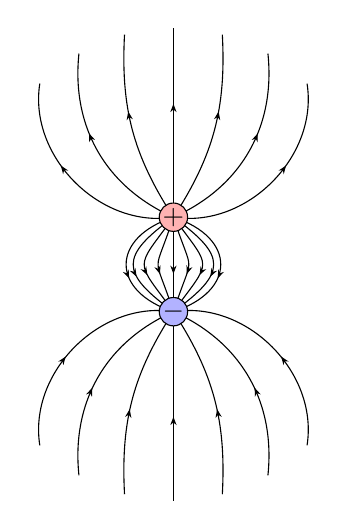
\begin{tikzpicture}[scale=0.6]
    %% 
    %% Dipole
    % \draw
    % (0,1) to (3,4)
    % (0,-1) to (3,4)
    % ;
    \foreach \X in {-4,...,4} 
    {
    \draw[postaction={decorate},decoration={markings,mark=at position 0.6 with {\arrow{Stealth[length=3pt]}}}] (0,1)  to[out={-90+\X*18},in={90+-\X*18},looseness=1.8]  (0,-1);
    }
    \foreach \X in {-3,...,3}
    {
    \draw[postaction={decorate},decoration={markings,mark=at position 0.6 with {\arrow{Stealth[length=3pt]}}}]  (0,1) to[bend left=18*\X] ++ (90+15*\X:4);
    \draw[postaction={decorate},decoration={markings,mark=at position 0.6 with {\arrow{Stealth[length=3pt, reversed]}}}]  (0,-1) to[bend left=18*\X] ++ (-90+15*\X:4);
    }
    % \draw[-Stealth] (0,0.7) to (0,-0.7);
    \draw[fill = red!30] (0,1) circle(0.3);
    \draw[fill = blue!30] (0,-1) circle(0.3);
    \draw
    (0,1) node{\(+\)}
    (0,-1) node{\(-\)}
    ;
    
\end{tikzpicture}    

\end{document}